\documentclass[t]{beamer}
% \usepackage{ulem}
\usepackage{pgf}
\usepackage{helvet}
\usepackage{calc}
\usepackage[utf8]{inputenc} % set your input encoding differently, if you want
\usepackage[english]{babel}

% Setting style of presentation
% =============================
\usetheme{NET}
\setbeamercovered{transparent=10}
\setbeamertemplate{navigation symbols}{}


% Some common packages
% ====================
\usepackage{units}
\usepackage{amsbsy}
\usepackage{amsmath}
\usepackage{amssymb}
\usepackage{amsthm}
\usepackage{wasysym}
\usepackage{graphics}
\usepackage{graphicx}
\usepackage{epsf}
\usepackage{epsfig}
\usepackage{fixmath}
% \usepackage{pgfmath}
\usepackage{wrapfig}
\usepackage{algorithm}
\usepackage{algpseudocode}
\usepackage{subfigure}

\DeclareMathOperator{\loca}{locate}
\newcommand{\hairspace}{\hspace{1pt}}
\newcommand{\eg}{\mbox{e.\hairspace{}g.,}\xspace}
\newcommand{\ie}{\mbox{i.\hairspace{}e.,}\xspace}
\newcommand{\Wlog}{\mbox{W.\hairspace{}l.\hairspace{}o.\hairspace{}g.}\xspace}


% \newtheorem{satz}{Satz}
% \newcommand{\myfont}{\Small}

% Adapt title information
% =======================
\title[OONIBear]{A new Crossbear hunter implementation}
\author[Ralph Holz, Jan Seeger, Vedat Levi Alev]{Ralph Holz, Jan Seeger, Vedat Levi Alev}
\institute{Network Architectures and Services \\ Technische Universität München}
\date{25.7.}


\begin{document}

\begin{frame}
  \titlepage
\end{frame}


%\begin{frame}
% \frametitle{Agenda}
% \begin{block}{}
%    \begin{itemize}
%      \item Starting point: X.509 vulnerabilities
%      \item Hunting the Men-in-the-middle: Crossbear
%        \begin{itemize}
%          \item Idea
%          \item Attacker model
%          \item Methods
%          \item Analysis and evaluation
%        \end{itemize}
%      \item Let's do SSH, too
%    \end{itemize}
% \end{block}
%\end{frame}



\begin{frame}
  \frametitle{X.509 PKI}
  \vskip -1cm
  \begin{block}{}
    \begin{figure}
      \centering
      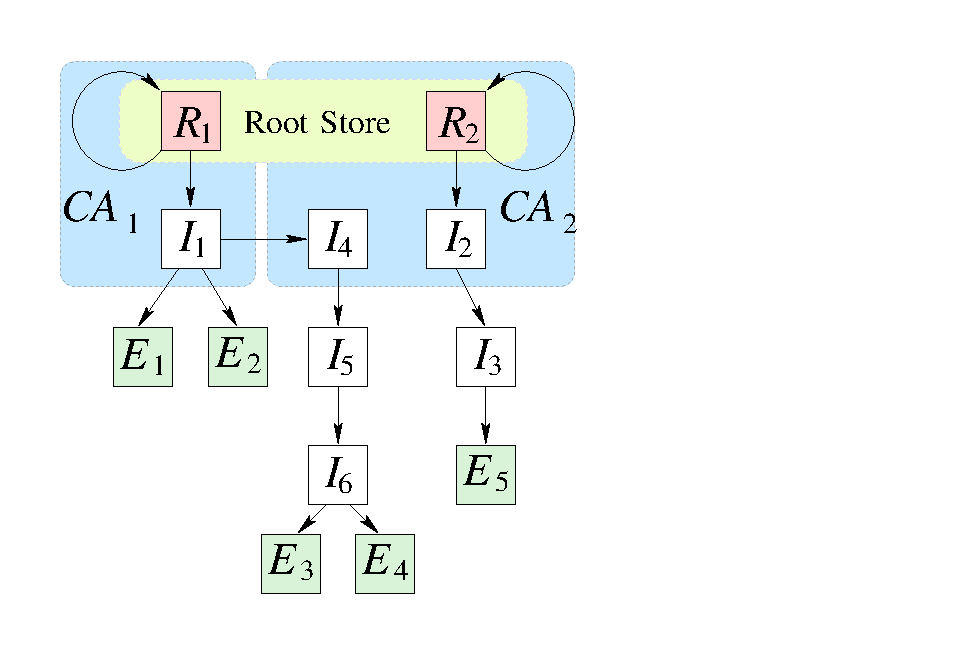
\includegraphics[scale=.7]{figures/x509tree-simplified.pdf}
    \end{figure}
  \end{block}
  \vskip -.7cm
  \begin{block}{\centering All CAs are created equal. Break one CA, break everything.}\end{block}
\end{frame}

\begin{frame}[fragile]
  \frametitle{Case study: DigiNotar}
\vskip -.8cm
    \begin{figure}
    \centering
     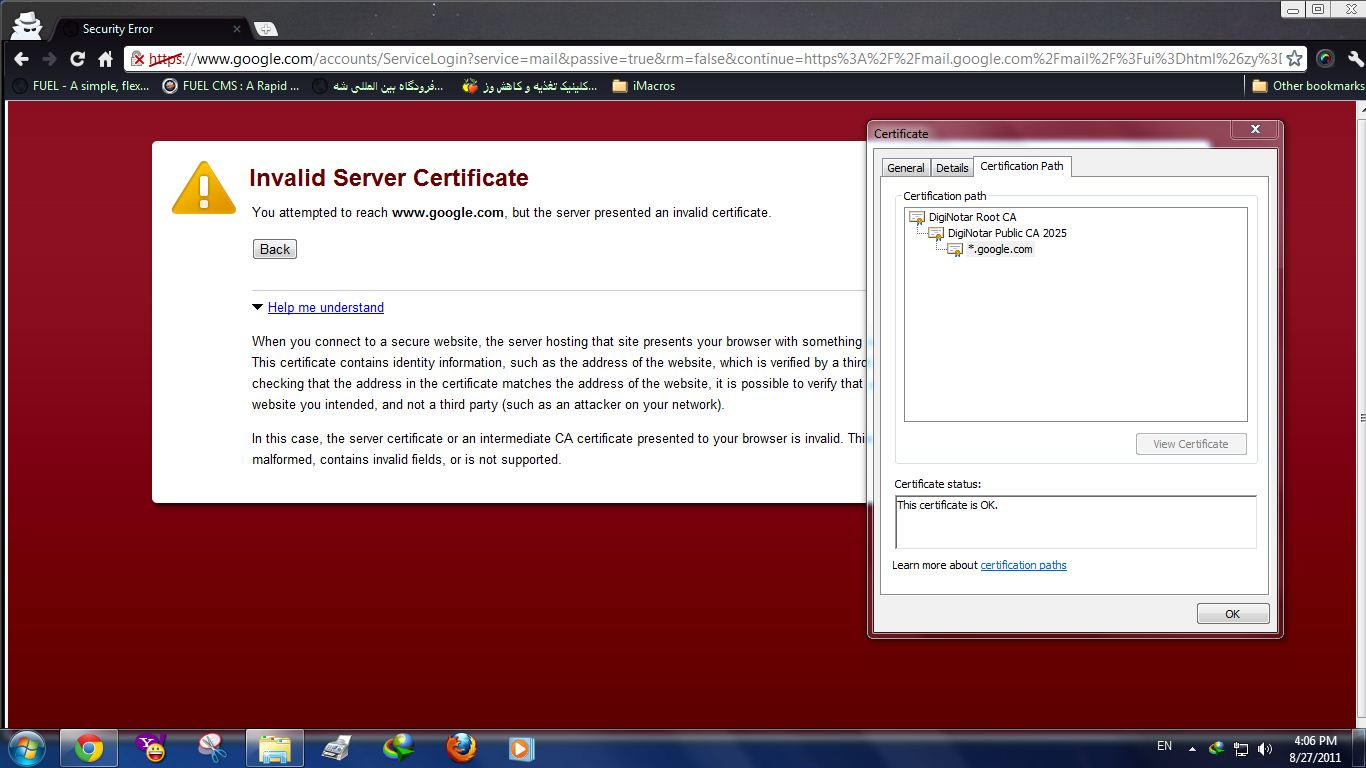
\includegraphics[scale=.37]{figures/gmail_iran.jpg}
    \end{figure}
\end{frame}

\begin{frame}
\frametitle{Crossbear: Hunting the MitM}
\begin{block}{This is \textit{not} a proposal to strengthen X.509.}\end{block}
\begin{block}{Crossbear: a tool to gather \textit{hard data}.}
  \begin{itemize}
    \item Raise reliable data about MitM \textit{in the wild}
    \item \textit{How often} do MitM attacks occur?
    \item \textit{Where} are the attackers located?
    \item \textit{Who} are the attackers?
  \end{itemize}
\end{block}
\begin{block}{Method: Combine notary principle, tracing and centralised reporting and analysis.}\end{block}
\end{frame}

%%% Local Variables:
%%% mode: latex
%%% TeX-master: "folien"
%%% End:

\begin{frame}
  \frametitle{Alice is surfing...}
  \begin{block}{}
    \vskip -1.2cm
    \begin{figure}[t]
      \centering
      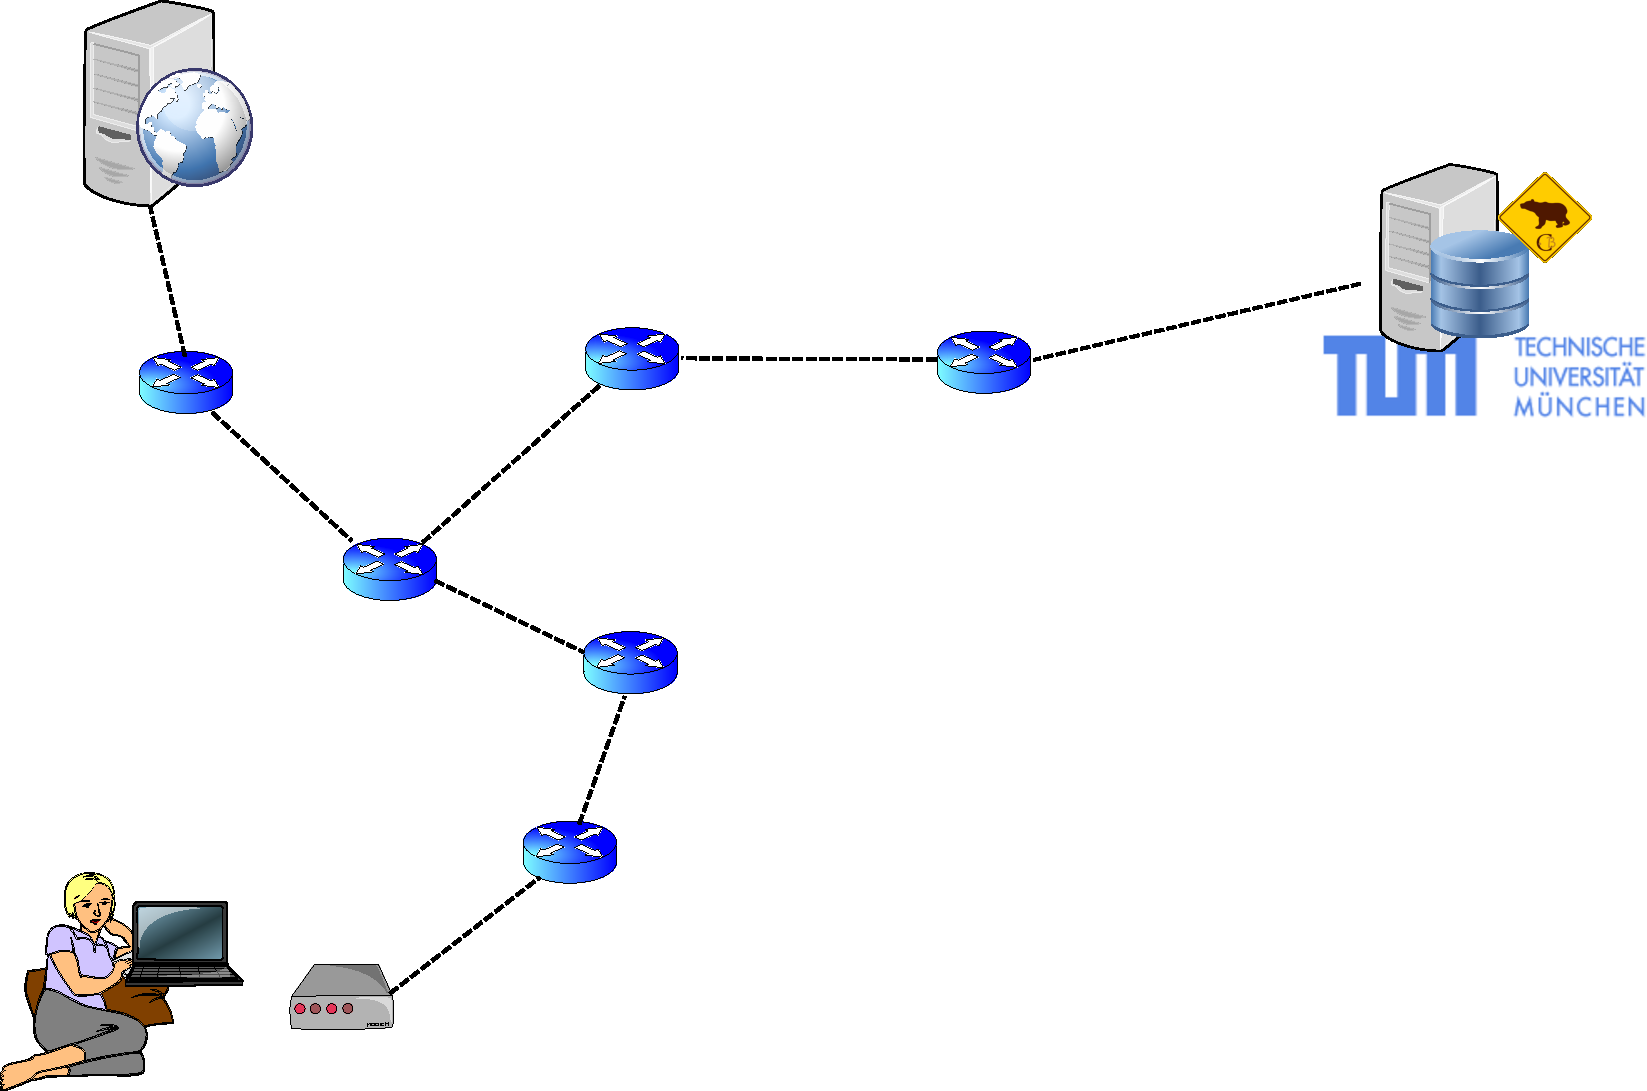
\includegraphics[scale=.36]{figures/reporting}
    \end{figure}
  \end{block}
\end{frame}

\begin{frame}
  \frametitle{Man-in-the-middle}
  \begin{block}{}
    \vskip -1.1cm
    \begin{figure}[t]
      \centering
      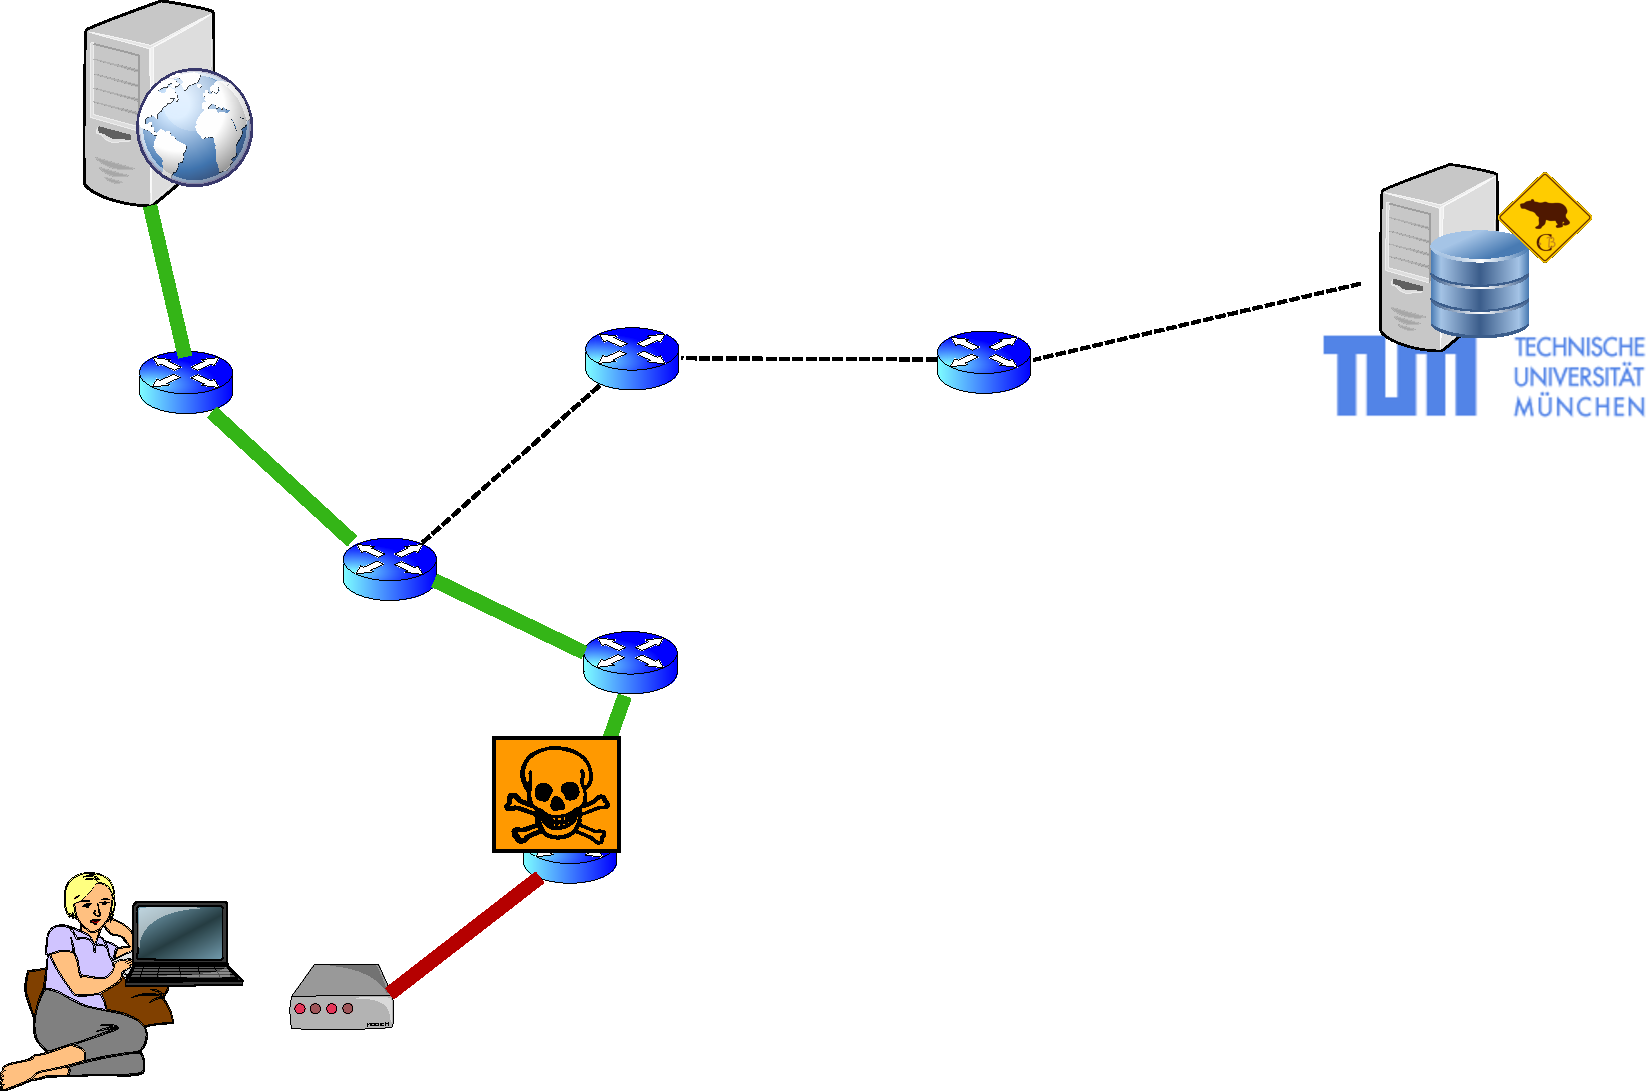
\includegraphics[scale=.36]{figures/reporting-2-attacked}
    \end{figure}
  \end{block}
\end{frame}

\begin{frame}
  \frametitle{Alice queries Crossbear}
  \begin{block}{}
    \vskip -1.2cm
    \begin{figure}[t]
      \centering
      \includegraphics[scale=.36]{figures/reporting-3-querying}
    \end{figure}
  \end{block}
  \vskip -.5cm
  \begin{block}{\small NB: SSL-secured connection, server cert hard-coded}\end{block}
\end{frame}

\begin{frame}
  \frametitle{Crossbear checks the server}
  \begin{block}{}
    \vskip -1.1cm
    \begin{figure}[t]
      \centering
      \includegraphics[scale=.36]{figures/reporting-4-checking}
    \end{figure}
  \end{block}
\end{frame}


\begin{frame}
  \frametitle{Crossbear reports result}
  \begin{block}{}
    \vskip -1.2cm
    \begin{figure}[t]
      \centering
      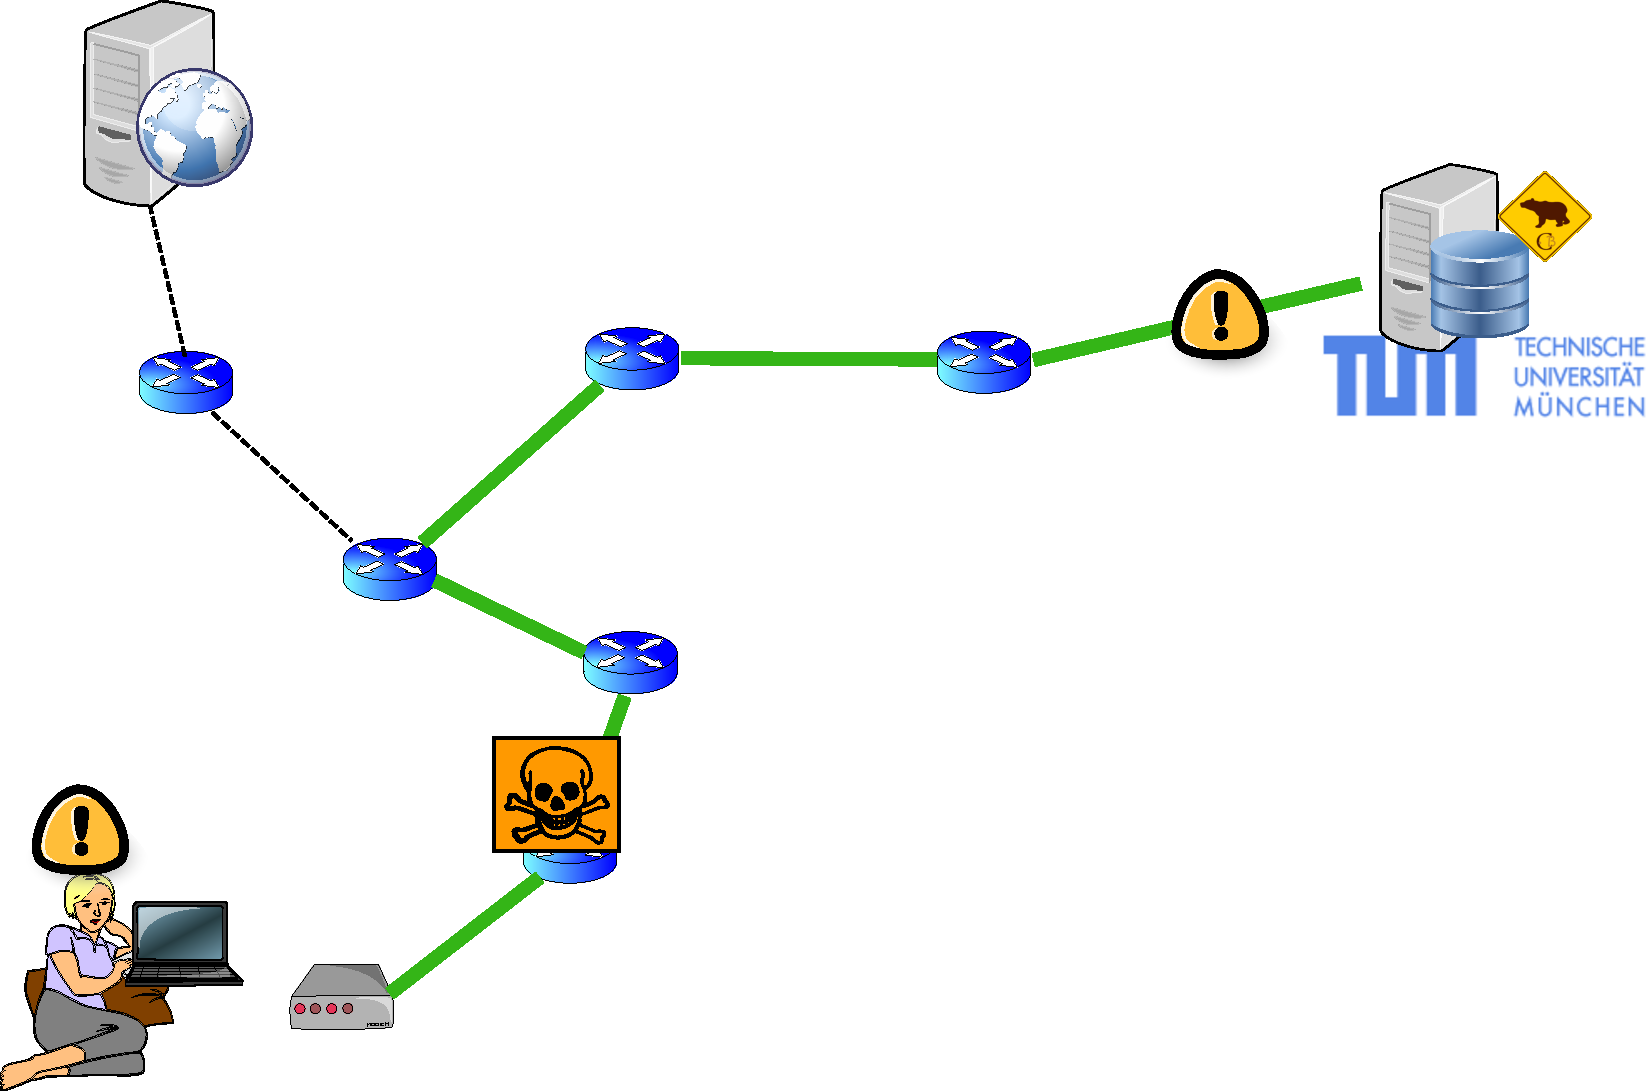
\includegraphics[scale=.36]{figures/reporting-5-feedback}
    \end{figure}
  \end{block}
\end{frame}


\begin{frame}
  \frametitle{Alice traceroutes to server}
  \begin{block}{}
    \vskip -1.1cm
    \begin{figure}[t]
      \centering
      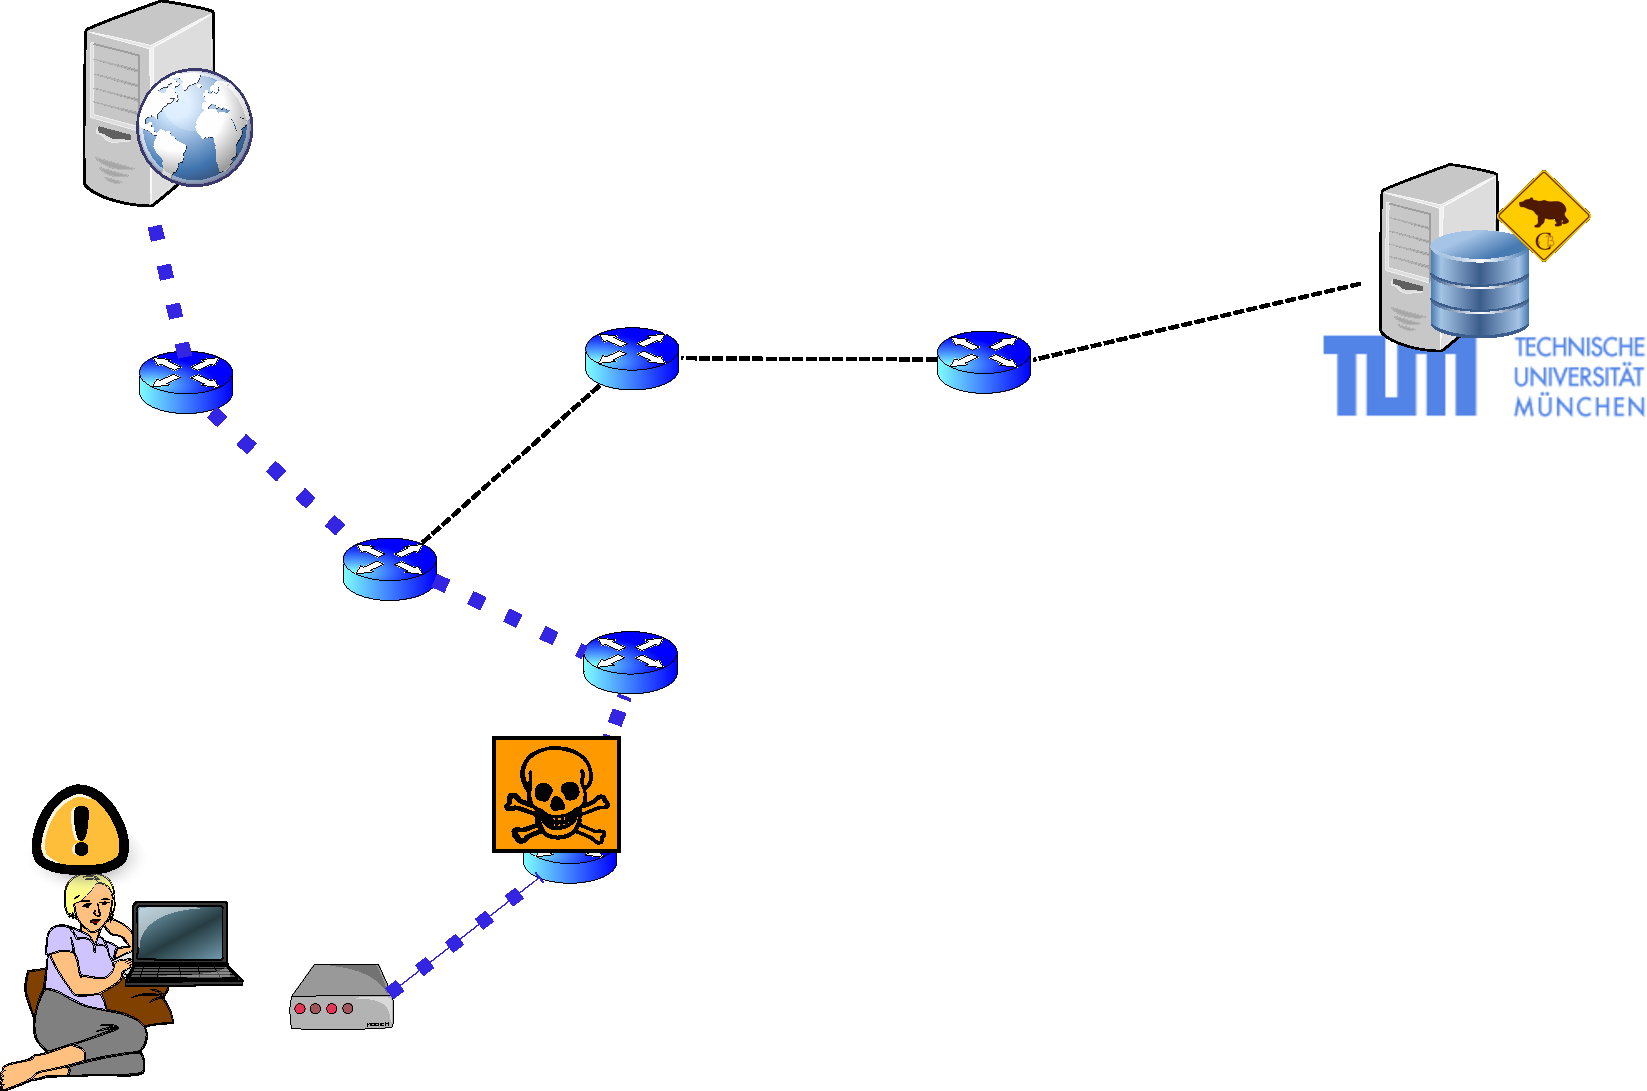
\includegraphics[scale=.36]{figures/reporting-6-hunting}
    \end{figure}
  \end{block}
\end{frame}


\begin{frame}
  \frametitle{Alice reports to Crossbear}
  \begin{block}{}
    \vskip -1.2cm
    \begin{figure}[t]
      \centering
      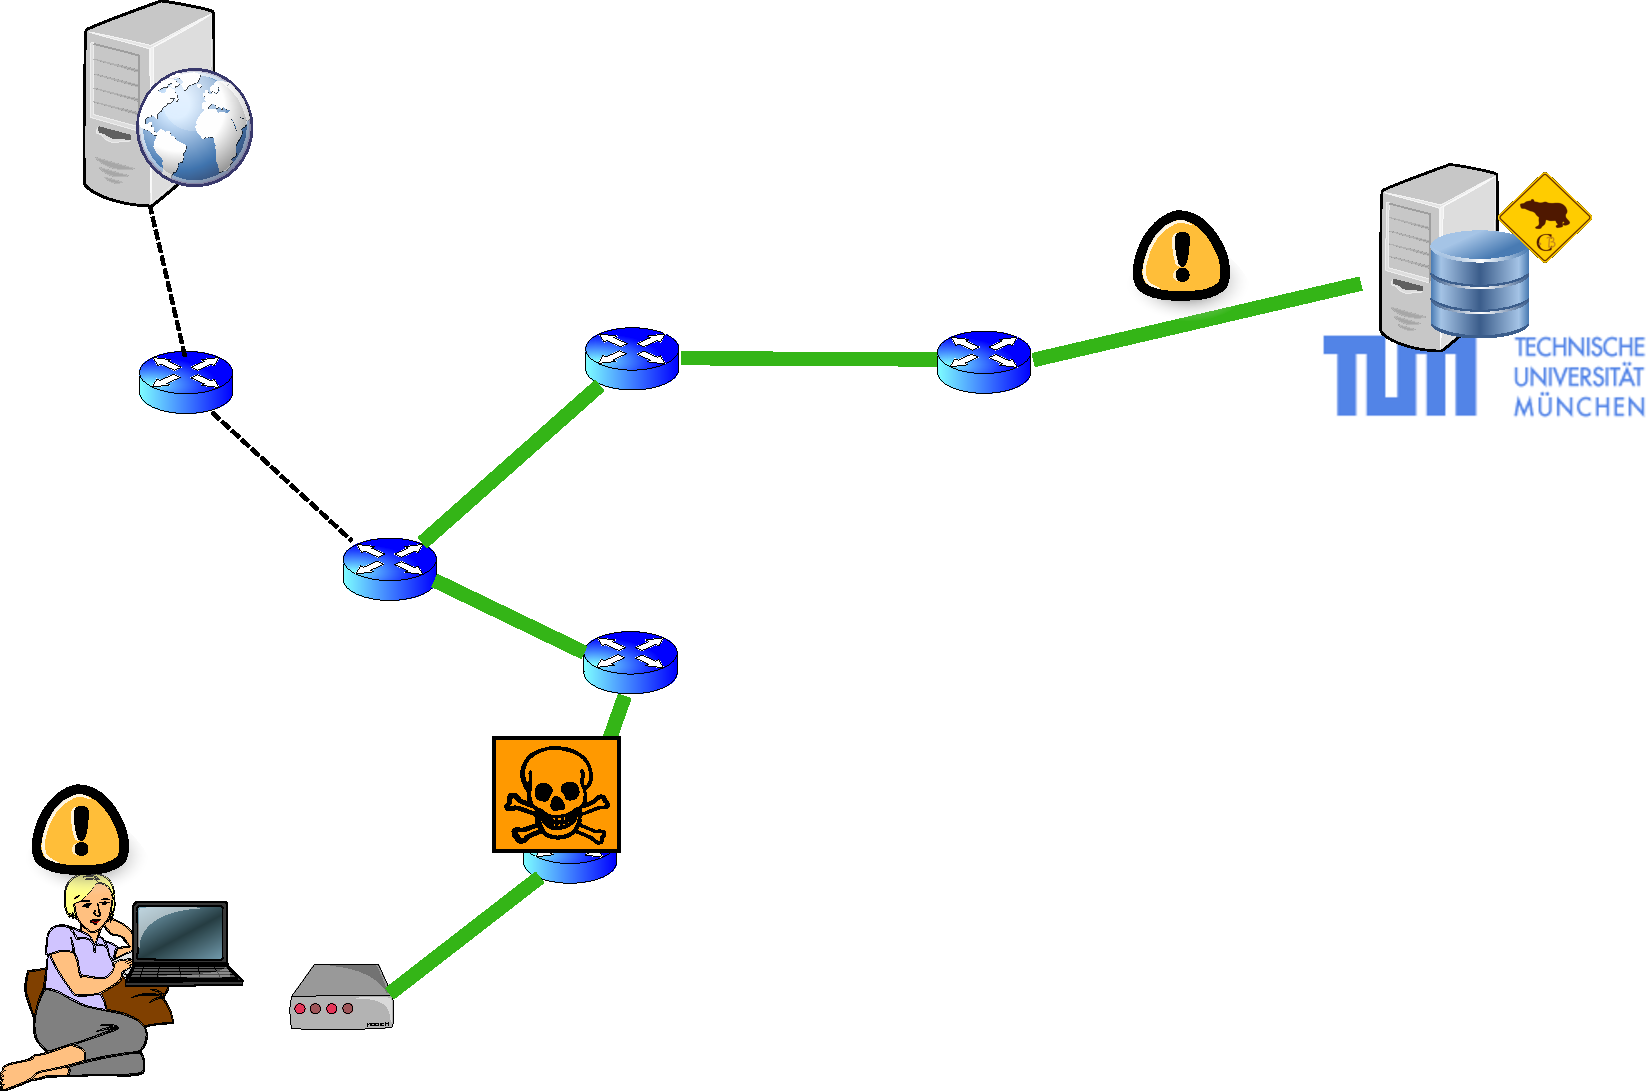
\includegraphics[scale=.36]{figures/reporting-7-huntingreport}
    \end{figure}
  \end{block}
\end{frame}

\begin{frame}
  \frametitle{Distribute hunting tasks}
  \begin{block}{}
    \vskip -1.2cm
    \begin{figure}[t]
      \centering
      \includegraphics[scale=.36]{figures/hunting-1-polling}
    \end{figure}
  \end{block}
\end{frame}

\begin{frame}
  \frametitle{Bob goes hunting}
  \begin{block}{}
    \vskip -1.2cm
    \begin{figure}[t]
      \centering
      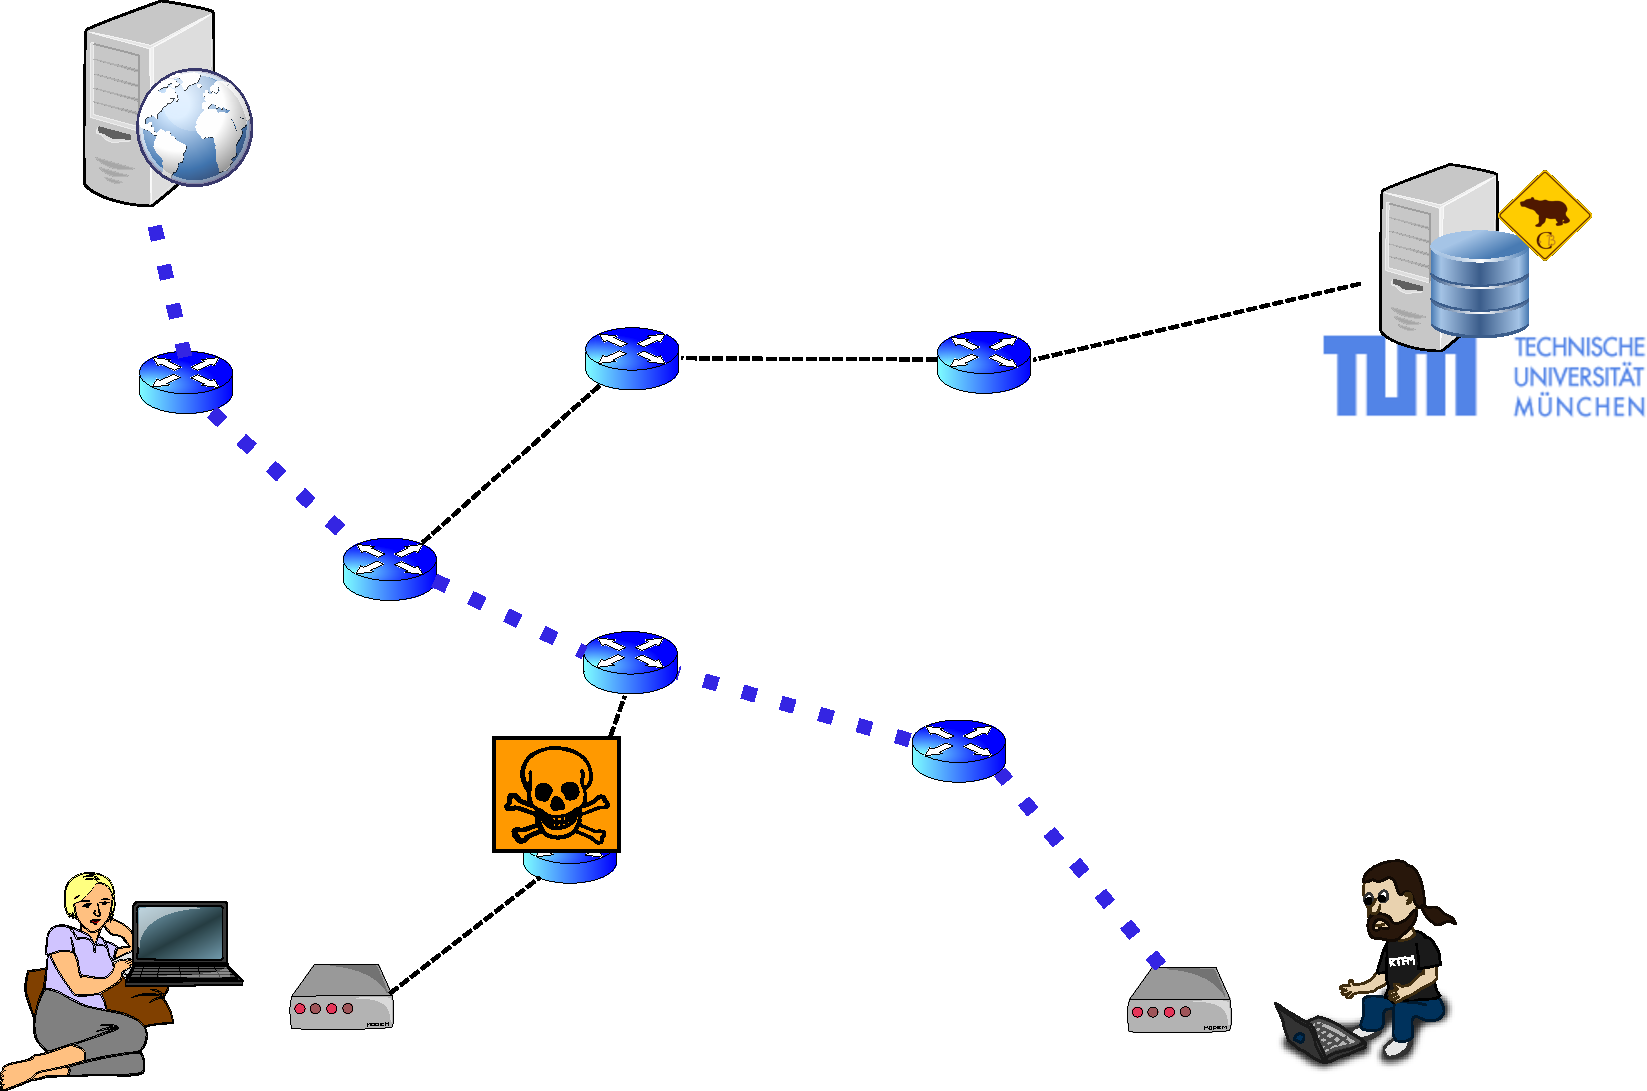
\includegraphics[scale=.36]{figures/hunting-2-hunting}
    \end{figure}
  \end{block}
\end{frame}

\begin{frame}
  \frametitle{Bob reports}
  \begin{block}{}
    \vskip -1.2cm
    \begin{figure}[t]
      \centering
      \includegraphics[scale=.36]{figures/hunting-3-reporting}
    \end{figure}
  \end{block}
\end{frame}

\begin{frame}
  \frametitle{There are many Bobs}
  \begin{block}{}
    \vskip -1.2cm
    \begin{figure}[t]
      \centering
      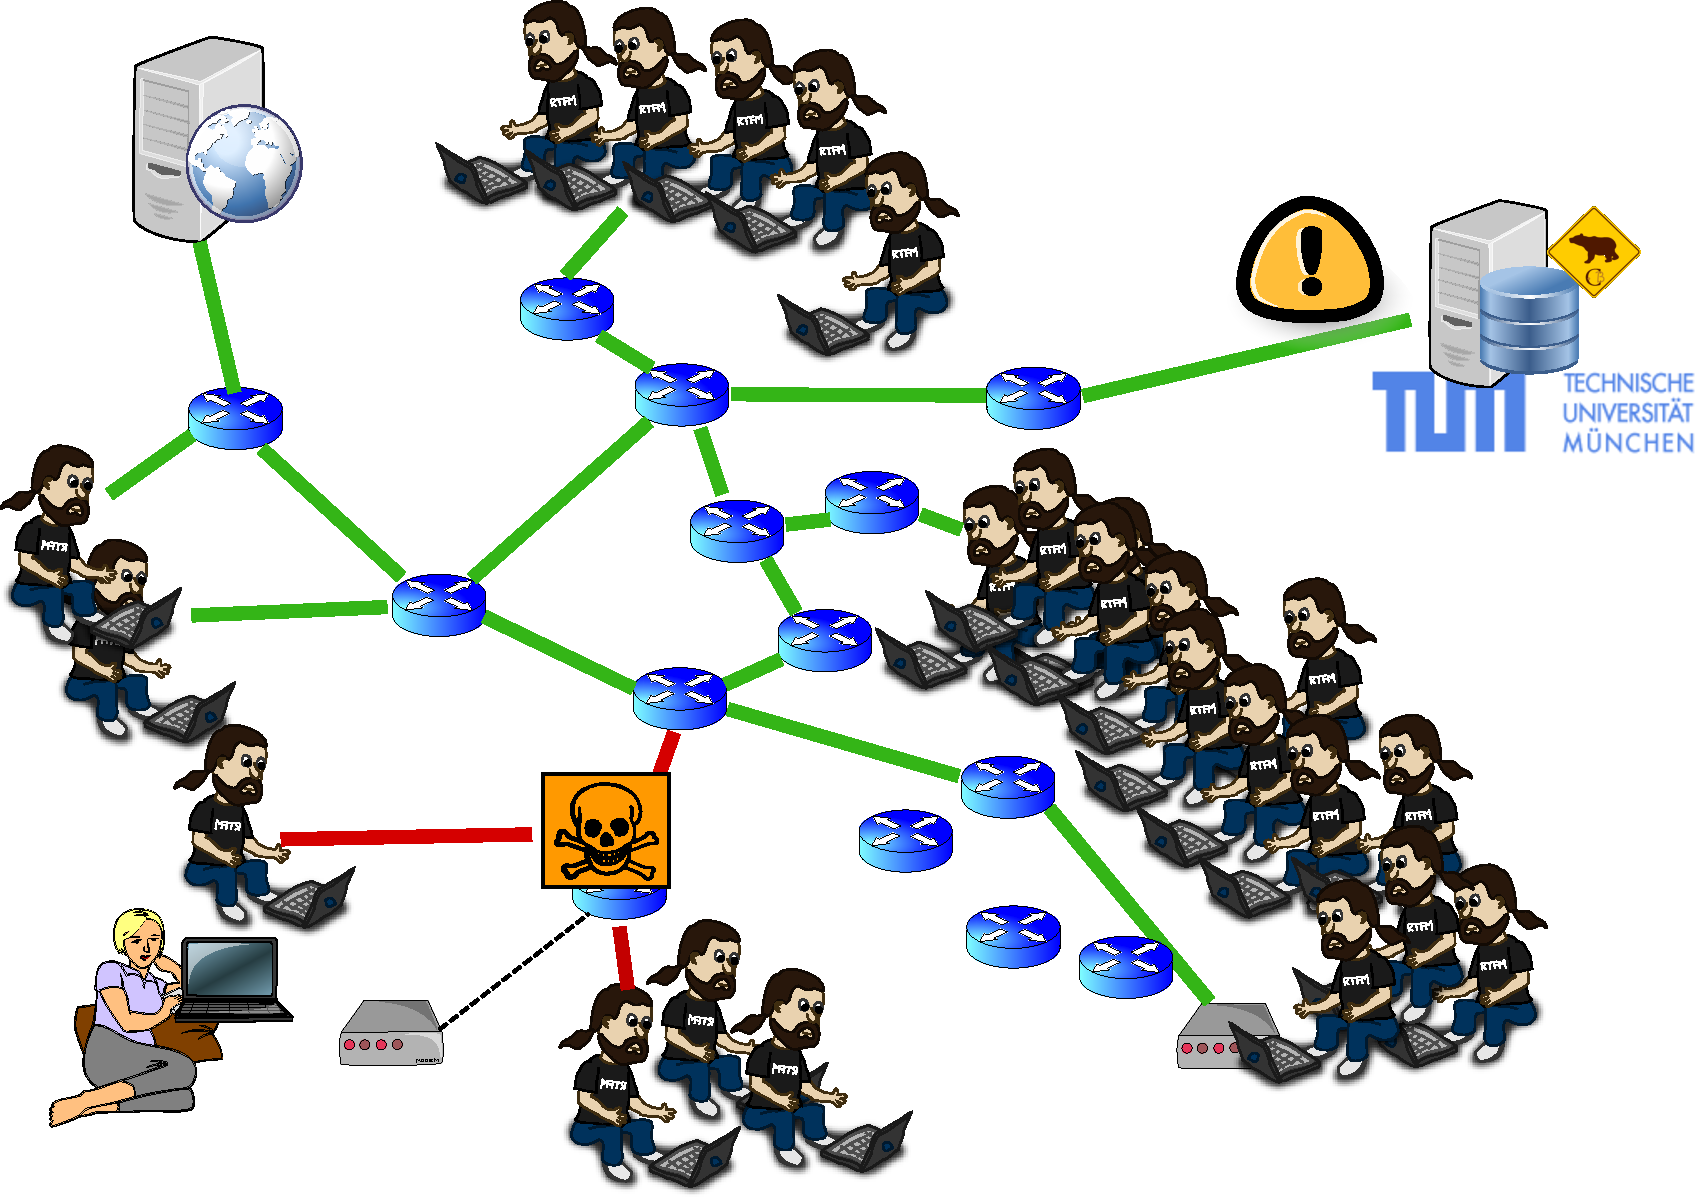
\includegraphics[scale=.36]{figures/hunting-4-manyreporting}
    \end{figure}
  \end{block}
\end{frame}

\begin{frame}
  \frametitle{Components}
  \begin{block}{Server: store and analyse}
    \begin{itemize}
    \item Crossbear server at TU M{\"u}nchen, Germany
    \item Additionally uses Convergence project's notaries
    \item Server cert hard-coded into client!
    \end{itemize}
  \end{block}
  \begin{block}{Clients}
    \begin{itemize}
    \item Firefox plugin (detection and localisation)
    \item Standalone hunting implementation (localisation only)
    \item OONIBear client (localisation only)
    \end{itemize}
  \end{block}
\end{frame}

\begin{frame}
  \frametitle{Additional data raised}
  \begin{block}{We also determine on server-side:}
    \begin{itemize}
    \item CAs used in certificate chain ($\rightarrow$ CA continuity)
    \item AS number of hosts in traceroute \\ ($\rightarrow$ Frequent
      reports about certain ASes?)
    \item Geo data: location of hosts in traceroute \\ ($\rightarrow$ Traversed countries)
    \item WHOIS info
    \end{itemize}
  \end{block}

  Also: Firefox add-on for \textit{detection} and \textit{hunting}.
\end{frame}

\begin{frame}
  \frametitle{OONIbear development}
  \begin{block}{What we did:}
    \begin{itemize}
    \item Port Crossbear client to Python
    \item Implement experimental IPv6 functionality
    \item Implemented analysers to gather additional data
    \end{itemize}
  \end{block}
  \begin{block}{What we still have to do:}
    \begin{itemize}
    \item Deeper integration into OONI
    \item Build a test setup for attacks
    \item Visualization tool for hunting results
    \end{itemize}
  \end{block}
\end{frame}

\begin{frame}
  \frametitle{Visualization mockup}
  \vspace{0.1\textheight}
  \begin{figure}[t]
    \centering
    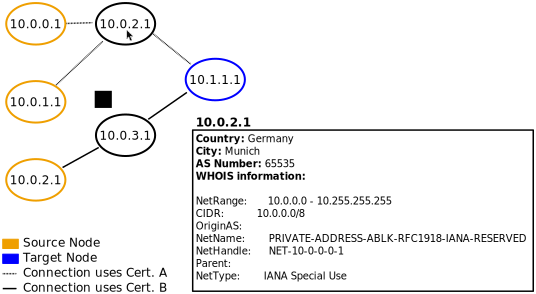
\includegraphics[width=.8\textwidth]{figures/Mockup-1}
  \end{figure}
\end{frame}

% \begin{frame}
%   \frametitle{Non-selective, close to victim client}
%   \begin{block}{}
%     \begin{figure}[t]
%       \centering
%       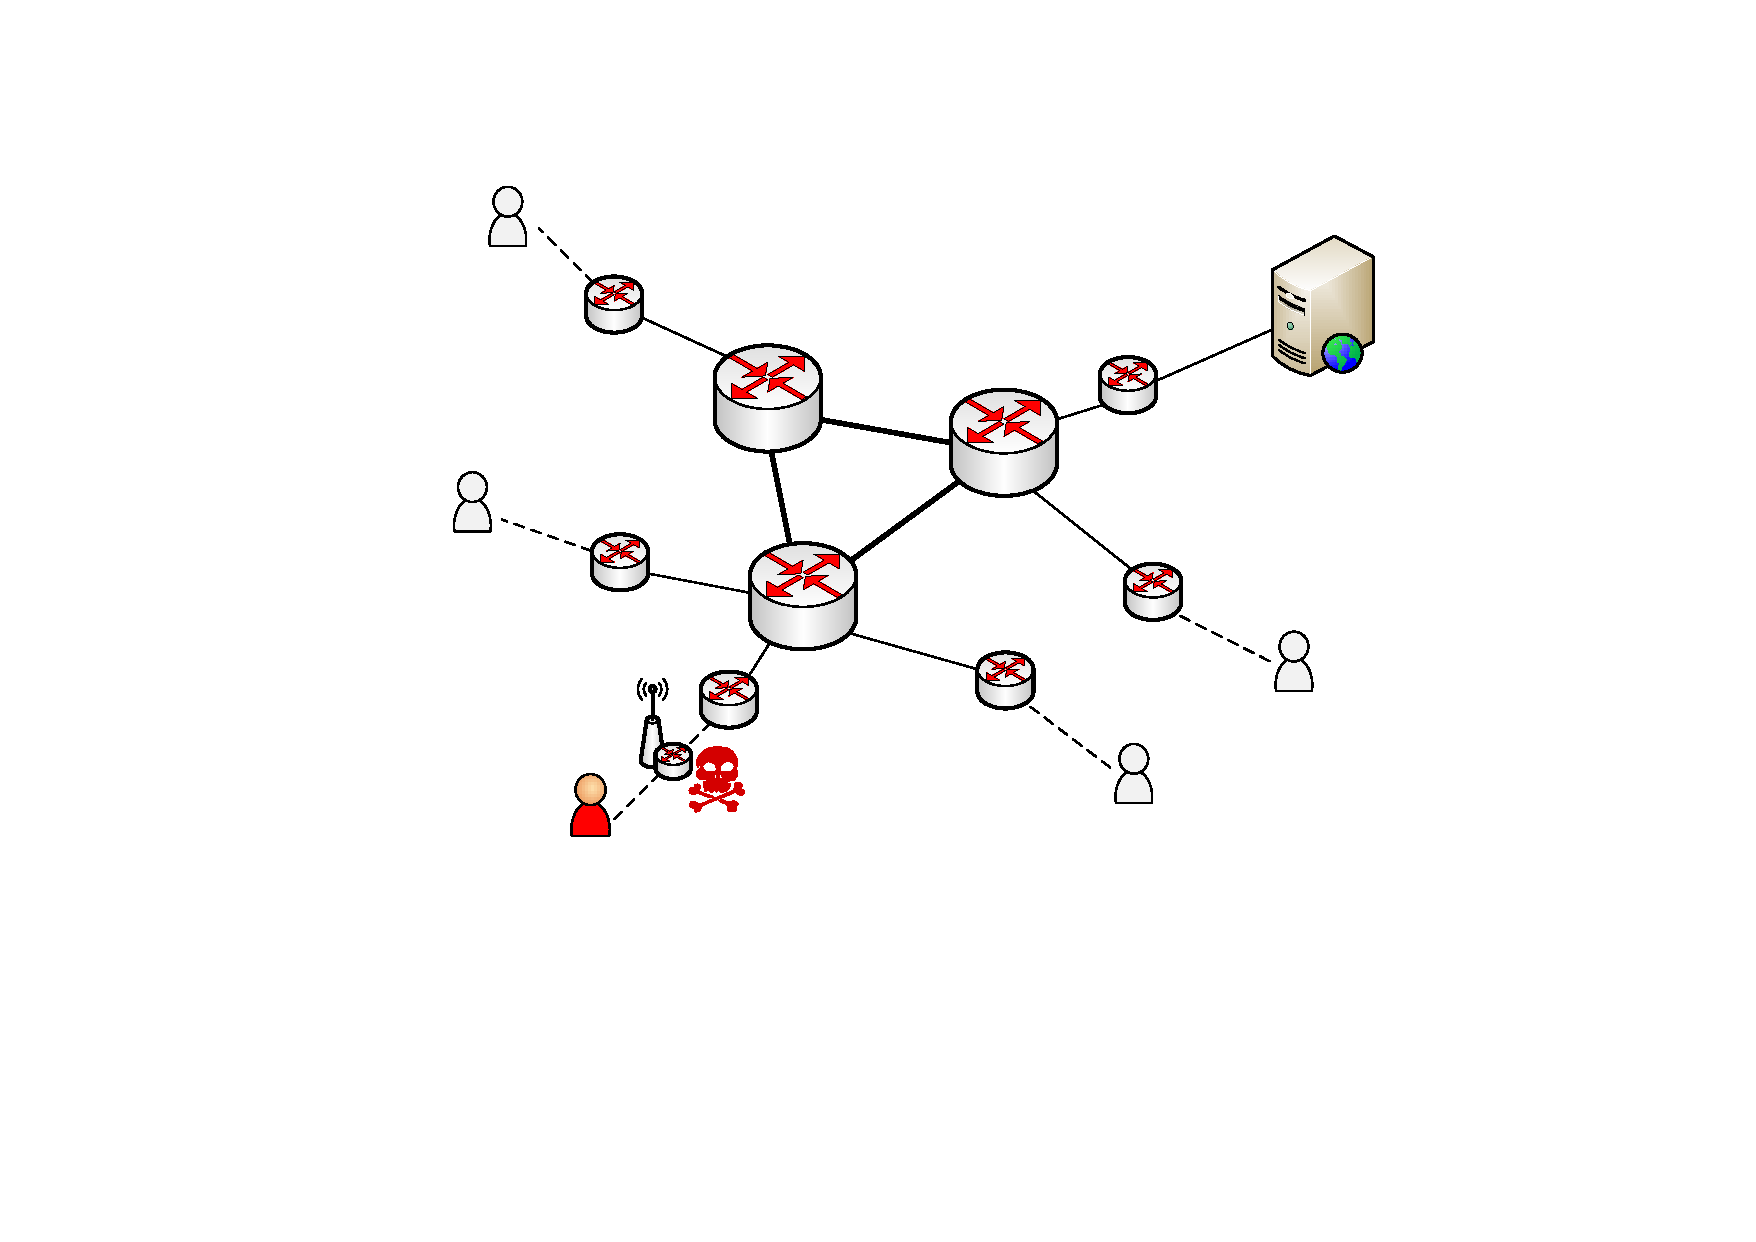
\includegraphics[scale=.5]{figures/scenario1-close-to-ap.pdf}
%     \end{figure}
%   \end{block}
% \end{frame}



% \begin{frame}
%   \frametitle{Non-selective, state-level attacker}
%   \begin{block}{}
%     \begin{figure}[t]
%       \centering
%       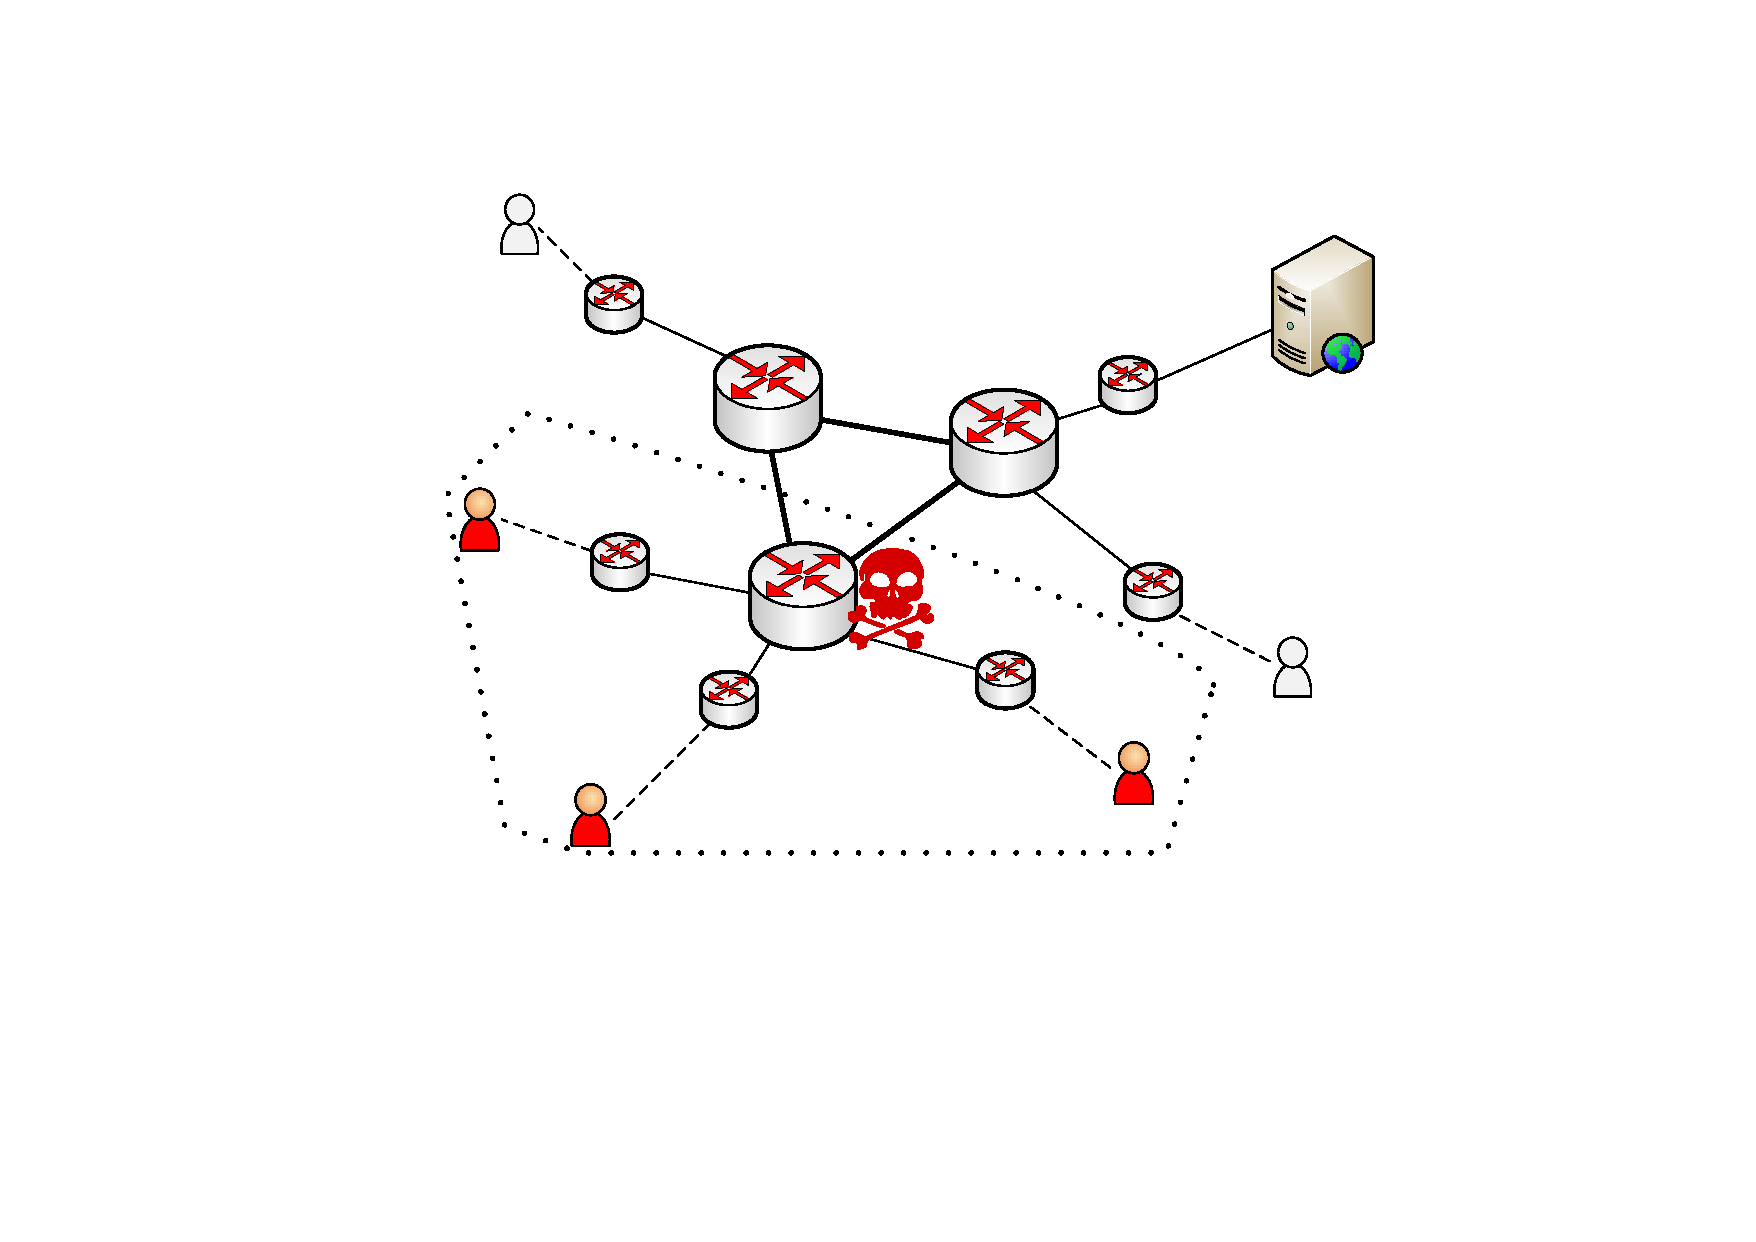
\includegraphics[scale=.5]{figures/scenario5-stateattacker-non-selective.pdf}
%     \end{figure}
%   \end{block}
% \end{frame}




% \begin{frame}
%   \frametitle{Analysis: non-selective attacker}
%   \begin{block}{Detection}
%     \begin{itemize}
%     \item Attack is detected if $\geq 1$ reports
% %     \item Attacker can only drop connections to Crossbear server
%     \end{itemize}
%   \end{block}
%   \begin{block}{Lends itself well to localisation}
%     \begin{itemize}
%     \item Get $\geq 1$ traceroute from victim,  $\geq 1$ from unpoisoned hunter 
%     \item The more, the better. The closer to intersection point, the better.
% %     \item Success depends on the number of hunters
%     \item An estimate can be given: \\ $<100$ hunters for $95\%$ accuracy on AS-level
%     \item Adaptive attackers are a problem (can't discuss here)
%     \item Full details in Crossbear research paper
%     \end{itemize}
%   \end{block}
% \end{frame}



% \begin{frame}
%   \frametitle{Number of hunters vs. success}
%   \vskip -.7cm
%   \begin{block}{}
%     \begin{figure}[t]
%       \centering
%       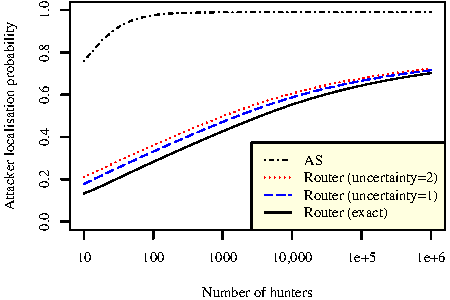
\includegraphics[scale=1.2]{figures/plot.pdf}
%     \end{figure}
%   \end{block}
%   \begin{block}{Imperfect, but given lack of data probably the best we can get.}\end{block}
% \end{frame}

\begin{frame}
  \frametitle{Thank you!}
  \vskip 1cm
  \begin{center}
    
\includegraphics[scale=0.2]{figures/question_mark.pdf}
  \end{center}
  \begin{block}{Contact}
    \begin{itemize}
    \item Twitter: @crossbearteam
    \item WWW: \texttt{https://pki.net.in.tum.de}
    \item \url{https://github.com/crossbear/Crossbear}
    \end{itemize}
  \end{block}
\end{frame}



\begin{frame}
  \frametitle{Selective attackers are a headache}
  \begin{figure}[t]
    \centering
    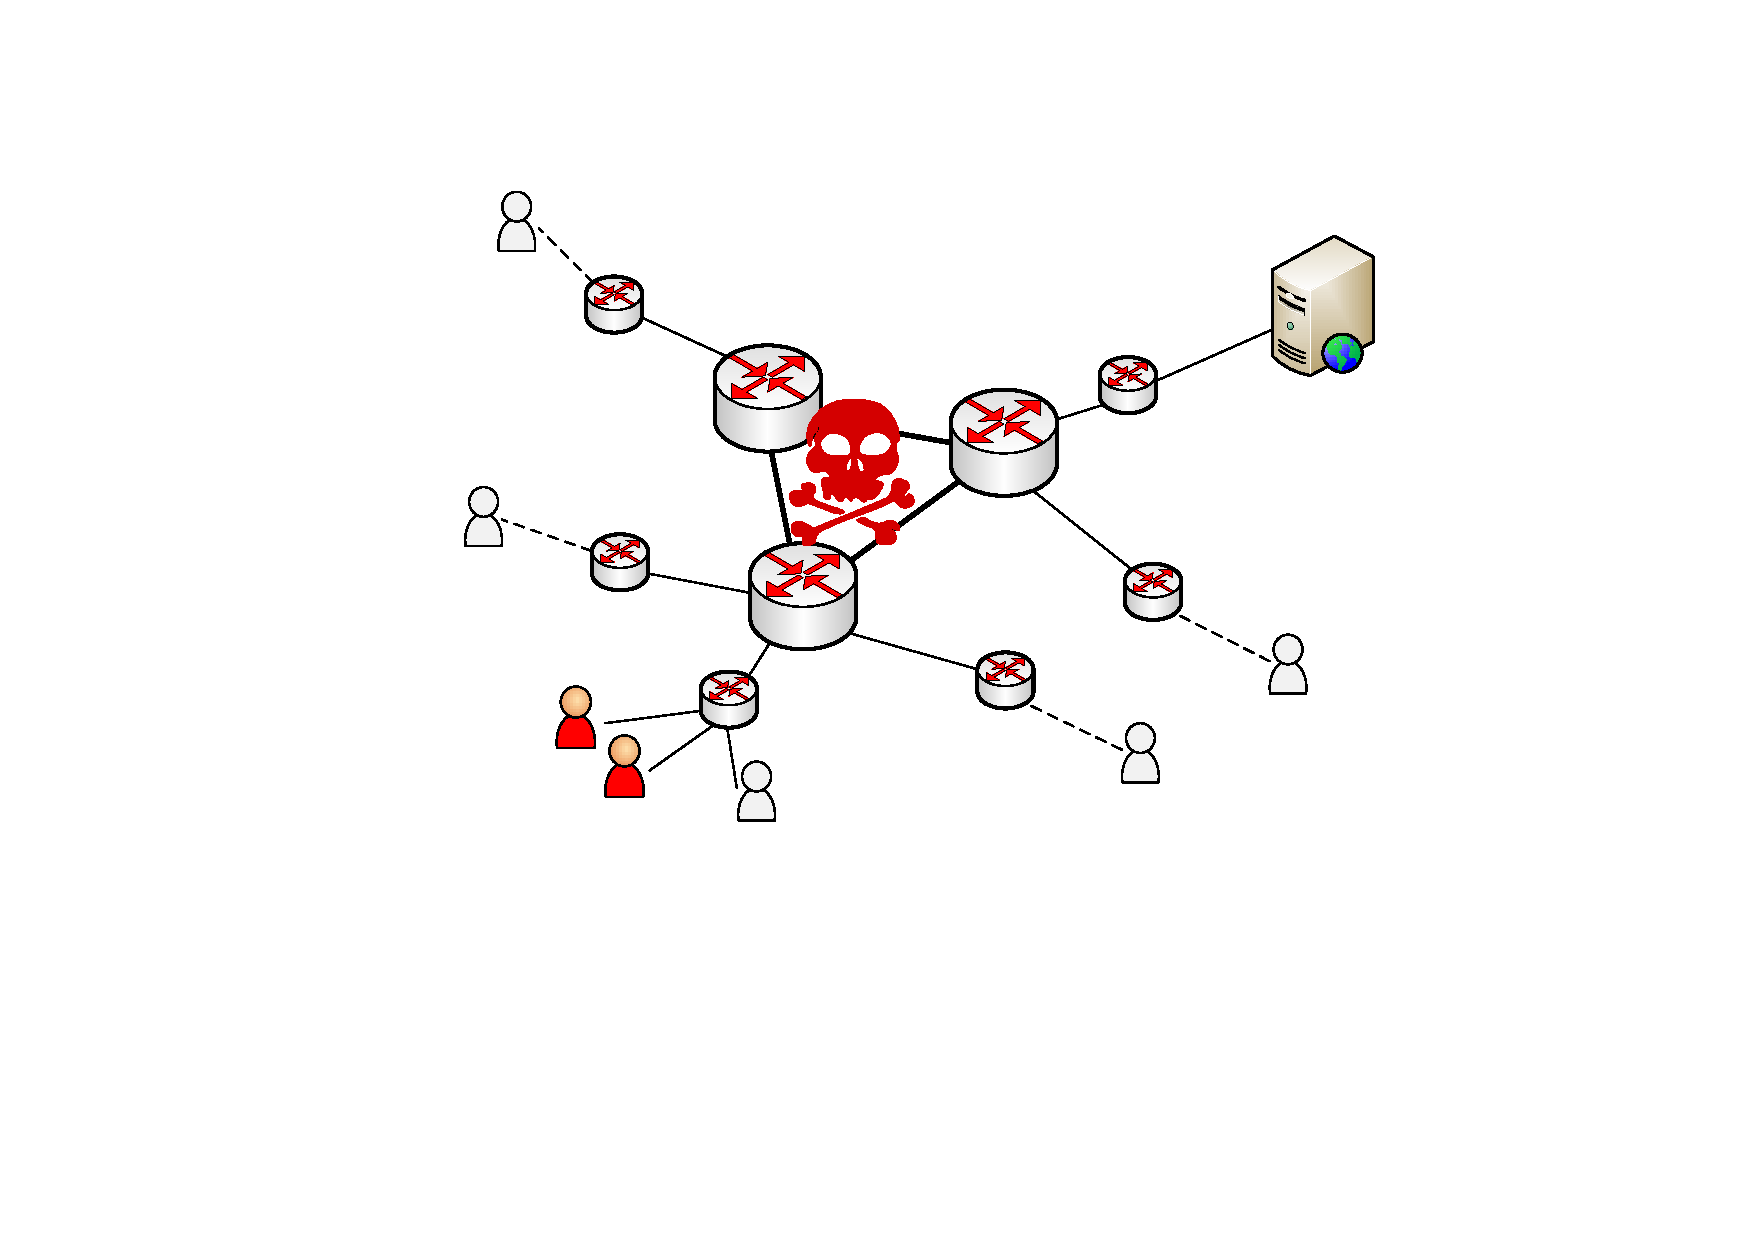
\includegraphics[scale=.3]{figures/scenario4-core-selective.pdf}
  \end{figure}
  \begin{block}{Can be indistinguishable from non-selective attacks}
    \begin{itemize}
    \item \textit{Every} attack report to be checked for plausibility
    \item But attacker should leave some hints -- cannot arbitrarily spoof IP addresses
    \end{itemize}
  \end{block}
\end{frame}



\begin{frame}
  \frametitle{Other issues}
  \begin{block}{Crossbear is an open system}
    \begin{itemize}
    \item Malicious injection of data
      \begin{itemize}
      \item Clients/hunters have no ID, no authentication
      \item Attacker can eclipse real hunters in his network, too
      \item Should results in clusters of suspicious reports, though
      \end{itemize}
    \item Denial-of-service attacks
    \item It is an arms race
    \item Other detection systems are subject to same attacks
    \end{itemize}
  \end{block}
\end{frame}

%%% Local Variables:
%%% mode: latex
%%% TeX-master: "folien"
%%% End:



%\part[Backup]{Backup Slides}
%\begin{frame}
%   \frametitle{}
%    \vskip 3cm
%    \begin{block}{\centering \huge Backup Slides}\end{block}
%\end{frame}

%\begin{frame}
  \frametitle{Surveys and solutions}
  \begin{block}{Talks and papers}
    \begin{itemize}
      \item Ristic: BlackHat 2010
      \item EFF: Defcon 2010
      \item Vratonjic et al., WPES, 2011
      \item Holz et al., IMC, 2011
    \end{itemize}
  \end{block}
  \begin{block}{They all agree: the system does not work, although some apologists remain.}\end{block}
\end{frame}


\begin{frame}
\frametitle{No silver bullet}
  \begin{block}{Scope of SSL/TLS:}
    \begin{itemize}
      \item Originally meant to protect things like credit card numbers
      \item State-scale attacks were not in scope back in the 1990s
    \end{itemize}
  \end{block}
  \begin{block}{Some proposals}
    \begin{itemize}
      \item Notary principle: Perspectives, Convergence
      \item Public Logs: Sovereign Keys, Certificate Transparency
      \item Keys in DNS(SEC): DANE, CAA
      \item Pinning
      \item PKI-me-harder
    \end{itemize}
  \end{block}
\end{frame}

\begin{frame}
  \frametitle{Errors in TLS Connection Setup}
  \begin{block}{Scans from Germany, Nov 2009 and Apr 2011}
    \begin{figure}
    \centering
      \includegraphics[scale=1.2]{plots/conn-err.pdf}
    \end{figure}
  \end{block}
\end{frame}


\begin{frame}
  \frametitle{Errors in TLS Connection Setup}
  \begin{block}{\texttt{UNKNOWN PROTOCOL}}
    \begin{itemize}
      \item Rescanned those hosts and manual sampling
      \item Always plain HTTP...
      \item ... and always an \texttt{index.html} with HTML 2 ...
      \item Hypothesis: old servers, old configurations
      \item More likely to happen in the lower ranks
    \end{itemize}
  \end{block}
\end{frame}

\begin{frame}
  \frametitle{Unusual Host Names}
  \begin{block}{CN=plesk or similar}
   \begin{itemize}
      \item Found in 7.3\% of certificates
      \item Verified: Plesk/Parallels panels
%       \item Verified: rescanned,  histograms of HTML replies
   \end{itemize}
  \end{block}
  \begin{block}{CN=localhost}
    \begin{itemize}
      \item 4.7\% of certificates
%       \item Very common: redirection to HTTP after HTTPs
    \end{itemize}
  \end{block}
\end{frame}


\begin{frame}
  \frametitle{Symmetric Ciphers}
  \begin{block}{Results from monitoring}
    \begin{figure}
    \centering
      \includegraphics[scale=.85]{plots/top-ciphers.pdf}
    \end{figure}
  \end{block}
  \begin{block}{(Mostly) in line with results from 2007 by Lee et al.}
   \begin{itemize}
    \item Order of AES and RC4 has shifted, RC4-128 most popular
   \end{itemize}
  \end{block}
\end{frame}


\begin{frame}
  \frametitle{Debian Weak Keys}
  \begin{block}{Weak randomness in key generation \\-- serious bug of 2008}
    \begin{figure}
    \centering
     \includegraphics[scale=.8]{plots/debian-weak-keys.pdf}
    \end{figure}
  \end{block}
  \begin{block}{In line with findings of 2009 by Yilek et al.}\end{block}
\end{frame}

\begin{frame}
  \frametitle{Public Key Lengths}
  \begin{block}{CDF for RSA key lengths -- linear Y axis}
    \begin{figure}
    \centering
     \includegraphics[scale=1.2]{plots/keylengths-times-linY.pdf}
    \end{figure}
  \end{block}
\end{frame}



\begin{frame}
  \frametitle{Public Key Lengths}
  \begin{block}{CDF for RSA key lengths -- double-log Y axis}
     \begin{figure}
    \centering
     \includegraphics[scale=1.2]{plots/keylengths-times-logY.pdf}
    \end{figure}
  \end{block}
\end{frame}



\begin{frame}
  \frametitle{Certificate Occurrences}
  \begin{block}{Most frequent Common Name occurrences}
    \begin{figure}
    \centering
      \includegraphics[scale=1.4]{plots/top-domains.pdf}
    \end{figure}
  \end{block}
\end{frame}



\begin{frame}
  \frametitle{Certificate Chains}
  \vskip -1.5cm
  \begin{block}{}
    \begin{figure}
      \centering
      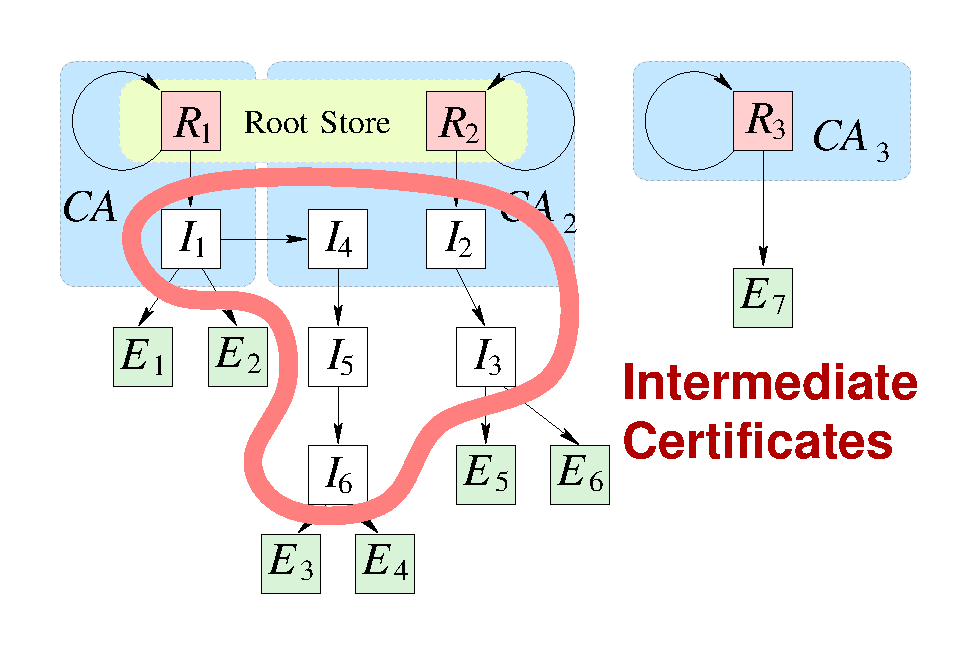
\includegraphics[scale=.7]{figures/x509tree-inter.pdf}
    \end{figure}
  \end{block}
\end{frame}




\begin{frame}
  \frametitle{Certificate Chain Lengths}
%   \vskip -1cm
%   \begin{columns}
%   \column{.5\textwidth}
    \begin{figure}
    \centering
      \includegraphics[scale=.9]{plots/chain-lengths.pdf}
    \end{figure}
%   \column{.5\textwidth}
%     \begin{figure}
%     \centering
%       \includegraphics[scale=.75]{plots/certchains-and-intermediates.pdf}
%     \end{figure}
%   \end{columns}
  \begin{block}{Finding more positive than negative:}
    \begin{itemize}
      \item Trend to use intermediate certificates more often
      \item Allows to keep Root Certificates offline
      \item But chains still reasonably short
   \end{itemize}
  \end{block}
\end{frame}

\begin{frame}
  \frametitle{Certificate Issuers}
  \begin{block}{Very few CAs account for $>$ 50\% of certificates}
    \begin{figure}
    \centering
     \includegraphics[scale=1]{plots/top-issuers.pdf}
    \end{figure}
  \end{block}
  \begin{block}{But there are 150+ Root Certificates in Mozilla.}\end{block}
\end{frame}


\end{document}
